\label{key}\documentclass[letterpaper, 12pt,oneside]{article}
\usepackage{amsmath}
\usepackage{graphicx}
\usepackage{xcolor}
\graphicspath{{Imagenes/}}
\usepackage[utf8]{inputenc}
\usepackage{listings}
\usepackage[hidelinks]{hyperref}

\title{\Huge Taller de Herramientas Computacionales}
\author{Josué Artemio Hernández Rodríguez}
\date{24/Enero/2019}

\begin{document}
	\maketitle
	\begin{center}
		
\includegraphics[scale=0.7]{3.jpg}
	\end{center}

	\newpage
	
	\title{\huge \textit{Bitacora problema 3 }}\\
	
	Este problema convierte de grados F a grados C, y viceversa. Lo que implemente fue un tipo menú, que el programa me preguntara que quería convertir, de las dos opciones F-C o C-F, y ademas la cantidad de grados. Coloque un bucle \textit{if}, si la opción era 1 hiciera el respectivo calculo; y \textit{else} para el otro caso, que es la otra conversión.

	\begin{figure}[h]
		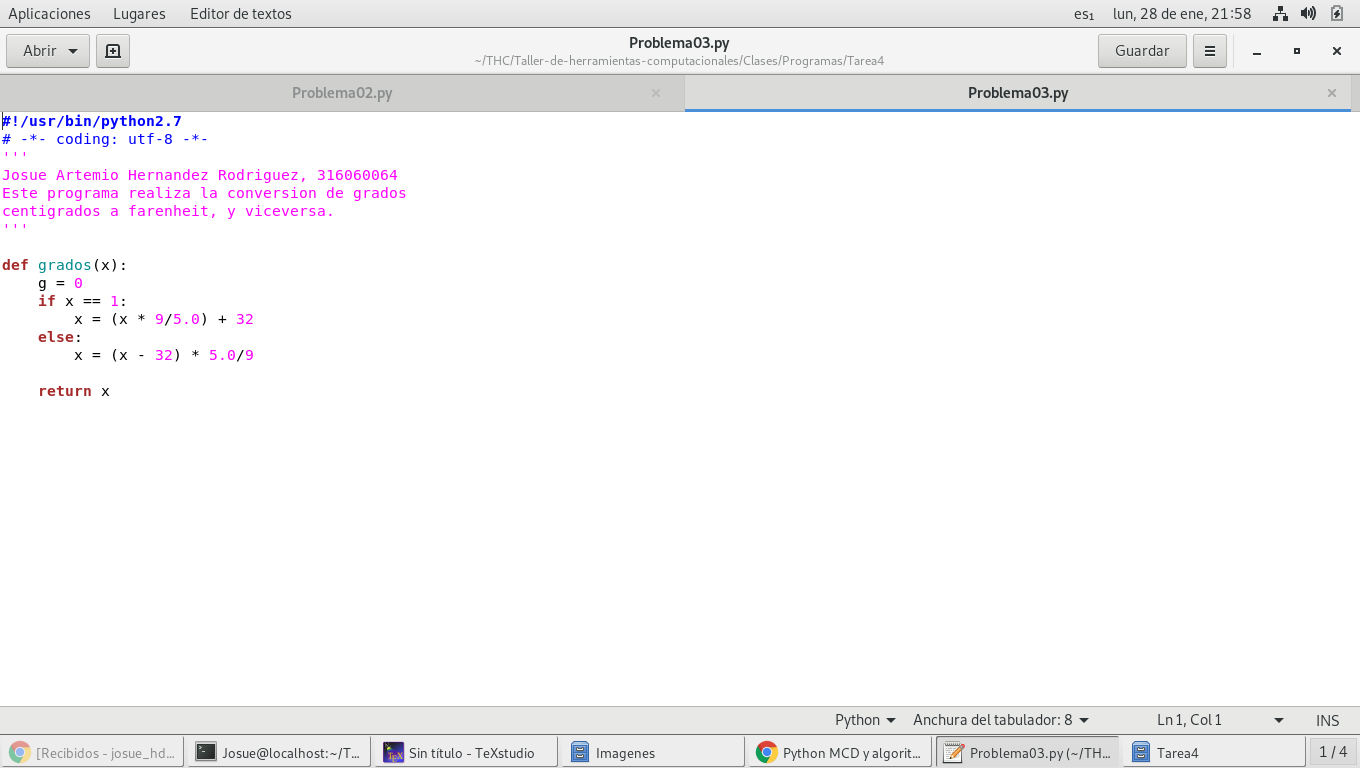
\includegraphics[scale=0.3]{pro03.png}
	\end{figure}
	
	
	
	
	
	
	
	
	
	
	
\end{document}
